% ============================================================
%  CHAPTER IV — RESULTS AND DISCUSSION
% ============================================================

\chapter{Results and Discussion}

This chapter presents the results of pipeline implementation across two case studies: the PHP codebase of FT UGM (Dashboard TCK) and the PHP codebase of DTI UGM (CBT System), along with a comparative analysis of the two. Each case study begins with a description of the dataset used, followed by the Rector conversion results, Semgrep scan results, PHPStan validation, and ISO/IEC 27001:2022 compliance mapping. The first case study also covers the five-LLM comparison experiment across three conditions and a composer dependency analysis. The closing section presents a comprehensive comparison of both case study results.

% ============================================================
\section{Case Study 1: FT UGM (Dashboard TCK)}
% ============================================================

% ------------------------------------------------------------
\subsection{Dataset Description}
% ------------------------------------------------------------

The first case study uses 245 PHP files from a single CodeIgniter 3.x-based internal web application managed by FT UGM. Its directory structure follows the standard CodeIgniter 3.x convention: \texttt{application/} for application code (controllers, models, views, helpers, configuration, services) and \texttt{system/} for framework code. The code was obtained through direct coordination with FT UGM and is used solely for static analysis in a local environment, with no access to the production database and no code execution.

Only \texttt{.php} files are processed; other files such as \texttt{.html}, \texttt{.js}, and \texttt{.css} are not copied to \texttt{output/} and are not analyzed. The dataset reflects characteristics common to legacy codebases: a mix of business logic, database access, and presentation within the same files, along with several PHP 5.x code patterns that persist even though the application overall runs on PHP 7.x.

For the LLM comparison experiment, 11 findings from the Semgrep pre-scan are used: 1 SQL Injection and 10 SSRF (Server-Side Request Forgery). These results constitute the entire pre-scan finding population, not a subjectively selected subset.

% ============================================================
\subsection{Rector Conversion Results}
% ============================================================

Rector was run against 245 PHP files from the FT UGM dataset with a target version of PHP 8.3. Of these 245 files, 239 were successfully converted, 4 were skipped, and 2 failed to process. The overall conversion rate ($CR = 97.6\%$) is shown in Figure~\ref{fig:rector-conversion}.

\begin{figure}[h]
    \centering
    
\includegraphics[width=0.8\textwidth]{contents/chapter-4/ft-ugm/pipeline_chart_mck_qwen_3_rector_conversion.png}
    \caption{Summary of Rector conversion results for 245 PHP files from the FT UGM dataset}
    \label{fig:rector-conversion}
\end{figure}
\newpage
Because the dataset contains a mix of PHP 5.x and PHP 7.x code, Rector automatically applies the cumulative ruleset chain from \texttt{UP\_TO\_PHP\_53} through \texttt{UP\_TO\_PHP\_83} in a single pass. This demonstrates that the pipeline can handle code from multiple PHP eras simultaneously without additional configuration.

\subsubsection{Examples of Rector Transformations}

To illustrate the types of changes performed by Rector, three representative transformations found in the FT UGM dataset are presented below.

\noindent\begin{minipage}{\linewidth}
\textbf{Transformation 1: Short array syntax (\texttt{ArrayShortSyntaxRector})}

In \texttt{system/core/Security.php}, array declarations using the old syntax are converted to the short syntax introduced in PHP 5.4:

\begin{lstlisting}[style=promptstyle]
// Before (PHP 7.x)
public $filename_bad_chars = array(
    '../', '<!--', '-->', '<', '>',
    "'", '"', '&', '$', '#',
);
protected $_never_allowed_str = array(
    'document.cookie' => '',
    'document.write'  => '',
);

// After (PHP 8.3)
public $filename_bad_chars = [
    '../', '<!--', '-->', '<', '>',
    "'", '"', '&', '$', '#',
];
protected $_never_allowed_str = [
    'document.cookie' => '',
    'document.write'  => '',
];
\end{lstlisting}
\end{minipage}

\noindent\begin{minipage}{\linewidth}
\textbf{Transformation 2: Null coalescing operator (\texttt{NullCoalescingRector})}

In \texttt{system/helpers/url\_helper.php}, the three-part \texttt{isset()} check pattern is converted to the more concise \texttt{??} operator:

\begin{lstlisting}[style=promptstyle]
// Before (PHP 7.x)
$atts[$key] = isset($attributes[$key])
    ? $attributes[$key] : $val;

// After (PHP 8.3)
$atts[$key] = $attributes[$key] ?? $val;
\end{lstlisting}
\end{minipage}

\noindent\begin{minipage}{\linewidth}
\textbf{Transformation 3: \texttt{str\_contains()} function (\texttt{StrContainsRector})}

In \texttt{system/helpers/url\_helper.php}, the substring search pattern using \texttt{strpos()} is converted to the \texttt{str\_contains()} function introduced in PHP 8.0. Rector also adds a \texttt{(string)} cast because the return value of \texttt{\$\_SERVER['SERVER\_SOFTWARE']} is of type \texttt{mixed} in PHP 8.x:

\begin{lstlisting}[style=promptstyle]
// Before (PHP 7.x)
if ($method === 'auto'
    && isset($_SERVER['SERVER_SOFTWARE'])
    && strpos($_SERVER['SERVER_SOFTWARE'],
        'Microsoft-IIS') !== FALSE)

// After (PHP 8.3)
if ($method === 'auto'
    && isset($_SERVER['SERVER_SOFTWARE'])
    && str_contains(
        (string) $_SERVER['SERVER_SOFTWARE'],
        'Microsoft-IIS'))
\end{lstlisting}
\end{minipage}

These three transformations reflect the most common categories of changes performed by Rector: syntax modernization, adoption of newer PHP APIs, and addition of type information required by PHP 8.x.

\subsubsection{Files That Failed Conversion}

Both files that failed conversion encountered the same internal error: the \texttt{FiberNodeScopeResolver::callNodeCallback()} function received a \texttt{null} argument where a \texttt{\detokenize{PhpParser\Node}} was expected. This is a bug in the version of Rector used, not a problem originating from the FT UGM source code.

The first file, \texttt{\detokenize{captcha_helper.php}}, contains a branching pattern that returns different data types — \texttt{GdImage} and \texttt{resource} — depending on the result of \texttt{\detokenize{function_exists()}} evaluation. Rector uses Fiber, a lightweight concurrency mechanism introduced in PHP 8.1, as the execution unit for analyzing each AST node separately during the transformation process \cite{phpgroup2022supported}. Under these conditions, the PHPStan Fiber used by Rector loses its reference to the AST node when analyzing a branch with such type differences.

The second file, \texttt{\detokenize{form_helper.php}}, contains more than 15 conditional function definitions wrapped in \texttt{\detokenize{if (!function_exists(...))}} constructs within the same file scope. The large number of analysis fibers running in parallel for each function creates a potential race condition, where one callback receives a node that has already been processed by another fiber.

Both files remain in the \texttt{\detokenize{output/}} directory as copies of the original code, so the conversion process retains all data without loss.

After conversion, all files in the \texttt{\detokenize{output/}} directory were tested for syntax validity using \texttt{\detokenize{php -l}}. The results showed no parse errors, giving a post-conversion syntax validity rate of 100\%.

% ============================================================
\subsection{Semgrep Security Scan Results}
% ============================================================

\subsubsection{Pre-Scan: Original Code Security Baseline}

The Semgrep scan against 241 PHP files in the \texttt{\detokenize{input/}} directory (out of the total 245 files; 4 files were excluded because they contain no PHP code analyzable by the Semgrep ruleset) produced 11 findings, comprising 1 SQL Injection vulnerability and 10 SSRF (Server-Side Request Forgery) vulnerabilities. All findings are localized to a single file: \texttt{\detokenize{Output.php}}.

The SQL Injection vulnerability was identified at line 768, where data from the \texttt{\detokenize{$_SERVER['QUERY_STRING']}} variable is used directly in cache path construction without appropriate sanitization. Additionally, 10 SSRF findings appeared in several locations within \texttt{\detokenize{Output.php}}. These findings arise from the use of filenames derived from user input in file system operations, opening the possibility of accessing unintended resources.

The concentration of all findings in a single file is indicative of a pattern common to legacy codebases, where the module handling output and caching tends to become a vulnerability hotspot due to its high level of interaction with external data that is not validated consistently.

\subsubsection{Post-Scan: Comparison After Conversion}

The Semgrep scan against the \texttt{\detokenize{output/}} directory after Rector conversion produced a finding count identical to the pre-scan: 11 findings. The security finding delta ($\Delta F = F_{post} - F_{pre} = 0$) shows no change. The distribution of vulnerability types also remained the same — 1 SQL Injection and 10 SSRF — all in the same file.

This result is consistent with expectations and indicates two things. First, the Rector conversion process did not introduce any new vulnerabilities into the FT UGM code. Second, the pre-existing vulnerabilities cannot be addressed through AST-based syntactic transformation, as they require fixes at the level of program logic (semantics), which falls outside the scope of that approach.

% ============================================================
\subsection{PHPStan Validation Results}
% ============================================================

PHPStan level 5 was run against the converted code in the \texttt{output/} directory targeting PHP 8.3. The result was 2,790 findings comprising 2,469 ERRORs and 321 WARNINGs, distributed across 179 of the 241 files analyzed. Among these findings, 354 are noise from the dynamic architecture of CodeIgniter 3 that PHPStan cannot analyze statically, including magic properties and helper functions injected at runtime.

Most of the errors found by PHPStan fall into three main categories. First, classes from third-party libraries that cannot be found, such as \texttt{PhpOffice\textbackslash\allowbreak PhpSpreadsheet} and \texttt{Dotenv\textbackslash\allowbreak Dotenv}: PHPStan cannot locate these classes because only the source code is analyzed, not the full application dependencies. Second, the use of return values from \texttt{void} functions as values — for example, \texttt{Result of method sendResponse() (void) is used} — a common pattern in legacy code written without explicit type declarations. Third, type inconsistencies such as \texttt{Cannot access property \$role on array}, reflecting the use of arrays as substitutes for typed objects without clear definitions.

These findings are manifestations of technical debt (accumulated code quality issues whose resolution has been deferred) that existed prior to migration, not errors introduced by the conversion process. PHP 8.3 has a far stricter type system than PHP 7.x, so problems that previously went undetected due to PHP 7.x's greater permissiveness are now surfaced by PHPStan. Figure~\ref{fig:phpstan-iso} shows the distribution of PHPStan findings by mapped ISO/IEC 27001:2022 control.

\begin{figure}[h]
    \centering
    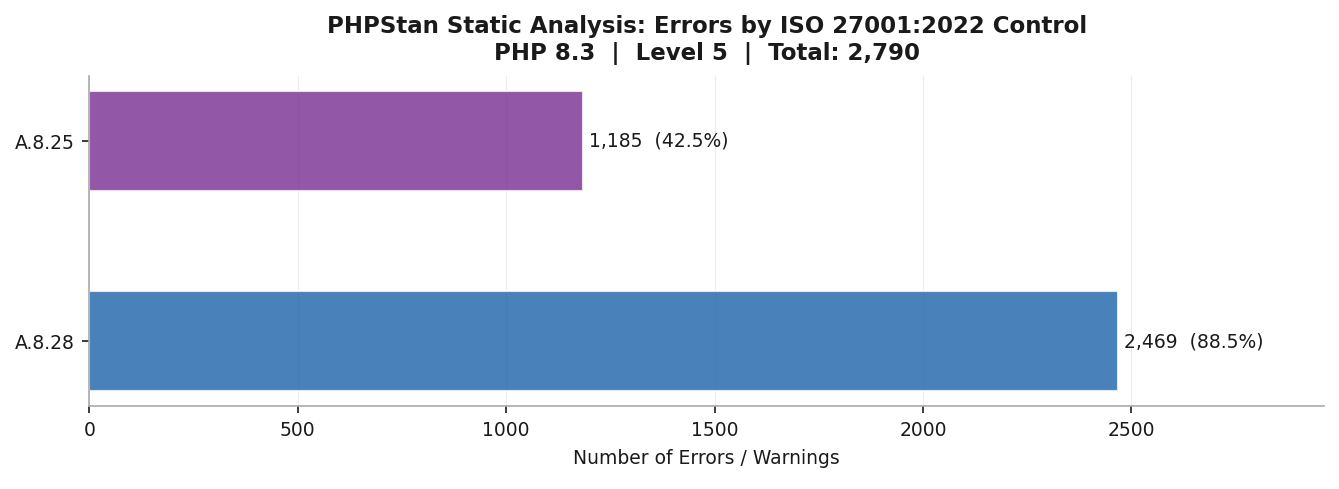
\includegraphics[width=1.0\textwidth]{contents/chapter-4/ft-ugm/pipeline_chart_mck_qwen_4_phpstan_iso.png}
    \caption{Distribution of PHPStan findings by ISO/IEC 27001:2022 Annex A control}
    \label{fig:phpstan-iso}
\end{figure}

The high PHPStan numbers actually demonstrate a concrete benefit of the validation component in this pipeline. Without PHPStan, these 2,790 potential type and compatibility issues would go undetected until the code runs in a production environment, consistent with the findings of Strobl et al. \cite{strobl2020automated} on the importance of automated quality assurance in large-scale code transformation.

% ============================================================
\subsection{ISO/IEC 27001:2022 Compliance Status}
% ============================================================

Based on the mapping performed by \texttt{iso\_mapper.py}, the compliance status for the six mapped ISO/IEC 27001:2022 controls is shown in Table~\ref{tab:iso-status}.

\begin{longtable}{|l|>{\raggedright\arraybackslash}p{2.5cm}|p{6cm}|p{3cm}|}
\caption{ISO/IEC 27001:2022 compliance status from the pipeline on the FT UGM dataset}
\label{tab:iso-status} \\
\hline
\textbf{Control} & \textbf{Title} & \textbf{Assessment Basis} & \textbf{Status} \\
\hline \hline
\endfirsthead

\multicolumn{4}{l}{\textit{(continued from Table \ref{tab:iso-status})}} \\
\hline
\textbf{Control} & \textbf{Title} & \textbf{Assessment Basis} & \textbf{Status} \\
\hline \hline
\endhead

\hline
\multicolumn{4}{r}{\textit{(continued on next page)}} \\
\endfoot

\hline
\endlastfoot

A.5.17 & Authentication Information &
No hardcoded credentials findings &
\texttt{COMPLIANT} \\
\hline

A.8.24 & Use of Cryptography &
No findings of \texttt{md5()}/\texttt{sha1()} used for password storage &
\texttt{COMPLIANT} \\
\hline

A.8.25 & Secure Development Lifecycle &
1,185 PHPStan findings in the \textit{undefined}/\textit{not found}
category mapped to this control &
{\footnotesize\ttfamily NON\_COMPLIANT} \\
\hline

A.8.26 & Application Security Requirements &
1 SQL Injection finding from Semgrep &
{\footnotesize\ttfamily NON\_COMPLIANT} \\
\hline

A.8.28 & Secure Coding &
Active Semgrep findings and 2,469 PHPStan ERRORs &
{\footnotesize\ttfamily NON\_COMPLIANT} \\
\hline

A.8.29 & Security Testing in Development &
\begin{minipage}[t]{6cm}10 open SSRF findings from Semgrep\end{minipage} &
{\footnotesize\ttfamily NON\_COMPLIANT} \\
\end{longtable}

The overall status is \texttt{NON\_COMPLIANT}. Finding counts per control in this table may exceed the total unique findings (2,790) because a single PHPStan finding can be mapped to more than one ISO control simultaneously. This result is consistent with the legacy code conditions analyzed, and objectively represents the security posture of the application prior to manual remediation.

The two controls with \texttt{COMPLIANT} status — A.5.17 and A.8.24 — must be understood in the appropriate context. This status means the Semgrep ruleset used produced no findings mapped to those two controls; it does not mean the code is entirely free of authentication or cryptography issues in an absolute sense.

Control A.8.29 has a \texttt{NON\_COMPLIANT} status because 10 active SSRF findings from Semgrep are mapped to this control and have not been addressed. Under the rule-based mapping mechanism defined in Section~\ref{sec:iso-mapping-design}, the presence of any active Semgrep finding on any control yields a \texttt{NON\_COMPLIANT} status, regardless of whether the pipeline has already executed automated security testing procedures. This compliance report is generated automatically and can be used directly as ISO/IEC 27001:2022 audit documentation \cite{iso27001_2022}.

% ============================================================
\subsection{Five-LLM Comparison Results (Condition A)}
% ============================================================

Having identified security vulnerabilities through Semgrep, the pipeline leverages the AI Engine component to formulate automated remediation suggestions for each finding. The Condition A experiment was run with an identical prompt for all models (zero-shot), 11 Semgrep pre-scan findings as input, 3 runs per finding per model, and a temperature of 0.1.
\subsubsection{Format Compliance Rate}

Figure~\ref{fig:format-compliance-a} shows the format compliance rate for each model in Condition A.

\begin{figure}[h]
    \centering
    
\includegraphics[width=1\textwidth]{contents/chapter-4/llm_chart_20260425_212836_2_format_compliance.png}
    \caption{Format compliance rate of the five LLM models in Condition A (zero-shot, identical prompt)}
    \label{fig:format-compliance-a}
\end{figure}

CodeLlama was the only model that consistently followed the prompt's format instructions across all 33 trials (100\%). DeepSeek Coder followed the format in 5 of 33 trials (15\%). Mistral followed the format in 2 of 33 trials (6\%). Qwen2.5-Coder and Llama 3.1 produced no responses that satisfied all three format elements simultaneously.

\subsubsection{Syntax Validity Rate}

Figure~\ref{fig:syntax-validity-a} shows the syntax validity rate and code block extraction rate for each model.

\begin{figure}[h]
    \centering
    
\includegraphics[width=1\textwidth]{contents/chapter-4/llm_quality_chart_20260425_122619.png}
    \caption{Syntax validity rate and code block extraction rate of the five LLM models in Condition A}
    \label{fig:syntax-validity-a}
\end{figure}

The results reveal a picture that is the inverse of the format metric. CodeLlama, which achieved 100\% format compliance, produced syntactically valid PHP code in only 9 of the 33 extracted code blocks ($SVR = 27.3\%$). This means 24 of the 33 CodeLlama code blocks contained parse errors.

Conversely, Qwen2.5-Coder, which achieved 0\% format compliance, successfully extracted PHP code blocks from 32 of 33 trials (97\%), and all 32 blocks passed \texttt{php -l} ($SVR = 100\%$). This model ignored the format instructions entirely but consistently produced high-quality code.

Mistral extracted 1 code block from 33 trials, but that block did not pass \texttt{php -l} (0\% validity). DeepSeek Coder and Llama 3.1 extracted 3 and 1 blocks respectively, each with 100\% validity, but the sample sizes are too small to be statistically representative.

\subsubsection{Summary Statistics}

Figure~\ref{fig:stats-table-a} summarizes the complete statistics for all five models in Condition A.

\begin{figure}[h]
    \centering
    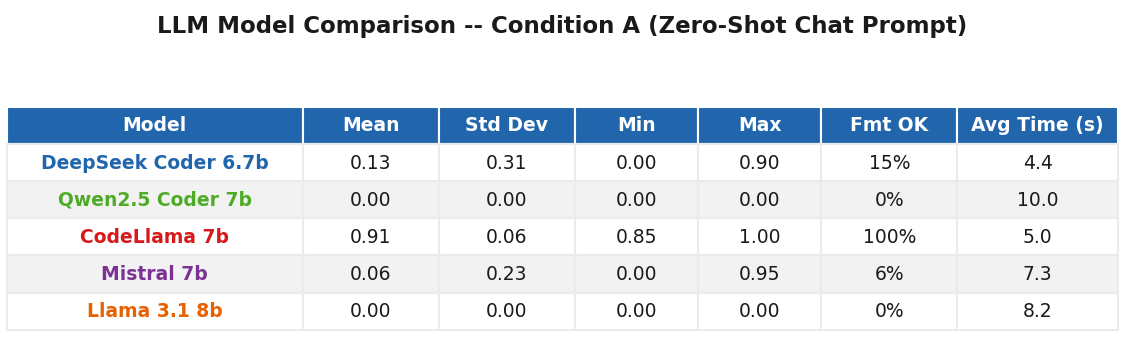
\includegraphics[width=\textwidth]{contents/chapter-4/llm_chart_20260425_203514_4_stats_table.png}
    \caption{Complete comparison statistics for the five LLM models in Condition A}
    \label{fig:stats-table-a}
\end{figure}

Statistics are computed from 33 inferences per model (11 findings $\times$ 3 independent runs, temperature = 0.1).

CodeLlama has a mean confidence score of $\bar{C}_m = 0.909$ with a standard deviation of $\sigma_m = 0.054$, reflecting high consistency within the narrow range $[0.85;\ 1.00]$. However, this consistency does not correlate with code quality: 72.7\% of CodeLlama's code is syntactically invalid, confirming that the self-reported confidence score is not a measure of code quality.

DeepSeek Coder recorded $\bar{C}_m = 0.132$ with a much larger standard deviation ($\sigma_m = 0.310$) and a range of $[0.00;\ 0.90]$. This high variance is consistent with the 15\% format compliance: only a small fraction of runs actually produced a \texttt{CONFIDENCE:} line, while the rest yielded a score of 0.0.

Mistral recorded $\bar{C}_m = 0.060$ with $\sigma_m = 0.230$ and a range of $[0.00;\ 0.95]$, a pattern similar to DeepSeek: high variance due to the infrequency of format-compliant responses.

Qwen2.5-Coder and Llama 3.1 both recorded $\bar{C}_m = 0.000$ with $\sigma_m = 0.000$. The 0.0 value arises when a response contains no pattern parseable by any of the six extraction patterns applied sequentially — neither a \texttt{CONFIDENCE:} line, a numeric expression, nor a natural language phrase such as \textit{"confident"} or \textit{"not sure"}. Specifically for Qwen2.5-Coder, the absence of a score does not indicate incapability; it reflects the model's response style of ignoring format instructions while still executing the primary task well. Qwen2.5-Coder's inference time (10.0 seconds) was the highest among all models, consistent with its longer and more detailed responses.

\newpage
\begin{lstlisting}[style=promptstyle]
$uri .= '?'.$_SERVER['QUERY_STRING'];
$cache_path .= md5(
    $CI->config->item('base_url')
    .$CI->config->item('index_page')
    .ltrim($uri, '/'));

if ( ! @unlink($cache_path)) {
    log_message('error',
        'Unable to delete cache file for '.$uri);
    return FALSE;
}
\end{lstlisting}

\textbf{CodeLlama response:}

\begin{lstlisting}[style=promptstyle]
VULNERABILITY: SQL Injection Vulnerability

The vulnerability is caused by the manual construction
of an SQL string, which allows user-controlled data
to be incorporated into the query. ...

SECURE PHP 8.x REPLACEMENT:
```php
$uri = $_SERVER['QUERY_STRING'];
$cache_path = md5(
    $CI->config->item('base_url')
    .$CI->config->item('index_page')
    .ltrim($uri, '/'));
if ( ! @unlink($cache_path)) {
    log_message('error',
        'Unable to delete cache file for '.$uri);
    return FALSE;
}
% (code block not closed, php -l fails)
\end{lstlisting}
\newpage
\textbf{Qwen2.5-Coder response:}
\begin{lstlisting}[style=promptstyle]
### Explanation of Vulnerability
...
Here's the corrected PHP 8.x code:
```php
$uri .= '?' . urlencode($_SERVER['QUERY_STRING']);
$cache_path .= md5(
    $CI->config->item('base_url')
    . $CI->config->item('index_page')
    . ltrim($uri, '/'));

if (!@unlink($cache_path)) {
    log_message('error',
        'Unable to delete cache file for '
        . urlencode($uri));
    return FALSE;
}
```
\end{lstlisting}

Several significant differences are evident from this comparison. CodeLlama correctly identifies the vulnerability but its solution is incorrect: the model only reformats the code without actually addressing the problem. The generated code still uses \texttt{\$\_SERVER['QUERY\_STRING']} directly with no sanitization.

Qwen2.5-Coder demonstrates deeper contextual understanding. The model recognizes that although Semgrep flagged this as SQL Injection, the code is actually constructing a cache path, not an SQL query. Its remediation suggestion uses \texttt{urlencode()} to prevent dangerous characters in the path. This is semantically more appropriate, although the ideal solution still requires review by a developer with full knowledge of the application context.

\subsubsection{Trade-offs and Implications}

From the overall Condition A results, a clear trade-off is evident between format compliance and code quality. The model most compliant with format instructions (CodeLlama, 100\%) produced code with the highest syntax error rate (72.7\% invalid code). The model producing the highest-quality code (Qwen2.5-Coder, 97\% extraction rate and 100\% validity) ignored the format instructions entirely.

This finding has a direct implication for the design of locally run LLM-based systems: code quality metrics (syntax validity rate) are a far more relevant indicator than format compliance metrics. An evaluation system that relies solely on format compliance will reach misleading conclusions about the practical utility of a model.

This trade-off also suggests that zero-shot conditions with an identical prompt may not be optimal for all models simultaneously, which provides the primary motivation for Condition B, where each model receives a prompt optimized based on the characteristics and weaknesses observed in Condition A.

% ============================================================
\subsection{Five-LLM Comparison Results (Condition B)}
% ============================================================

Condition B was designed to address the specific weaknesses of each model identified in Condition A. Each model receives a different prompt through the \texttt{\_build\_optimized\_chat\_messages()} method in \texttt{ai\_engine.py}, while the other experimental parameters remain identical: the same 11 Semgrep findings, 3 runs per finding per model, and a temperature of 0.1.

The optimization strategy for each model was formulated based on Condition A failure patterns. Qwen2.5-Coder received a more relaxed prompt without strict format requirements, since its code quality was already high. DeepSeek Coder received shorter, more direct instructions to reduce the complexity suspected of causing its low extraction rate. Mistral received one concrete few-shot example to demonstrate the expected output format. Llama 3.1 received explicit role-playing instructions with numbered steps. CodeLlama retained the Condition A format with an additional explicit instruction to produce syntactically valid PHP code.

\subsubsection{Format Compliance Rate}

DeepSeek Coder recorded the most significant improvement, rising from 15\% in Condition A to 61\% in Condition B. This confirms that the model is highly sensitive to instruction complexity: shorter, more direct prompts substantially improved its ability to follow the format. CodeLlama maintained 100\% format compliance as in Condition A. Conversely, Mistral regressed from 6\% to 0\%, and Llama 3.1 only rose slightly from 0\% to 3\% (1 of 33 runs).

Figure~\ref{fig:format-compliance-b} shows the format compliance rate for each model in Condition B.

\begin{figure}[h]
    \centering
    
\includegraphics[width=0.85\textwidth]{contents/chapter-4/llm_chart_20260427_130844_2_format_compliance.png}
    \caption{Format compliance rate of the five LLM models in Condition B (prompt optimized per model)}
    \label{fig:format-compliance-b}
\end{figure}

\newpage
\subsubsection{Syntax Validity Rate}

Figure~\ref{fig:syntax-validity-b} shows the syntax validity rate and code block extraction rate in Condition B.

\begin{figure}[h]
    \centering
    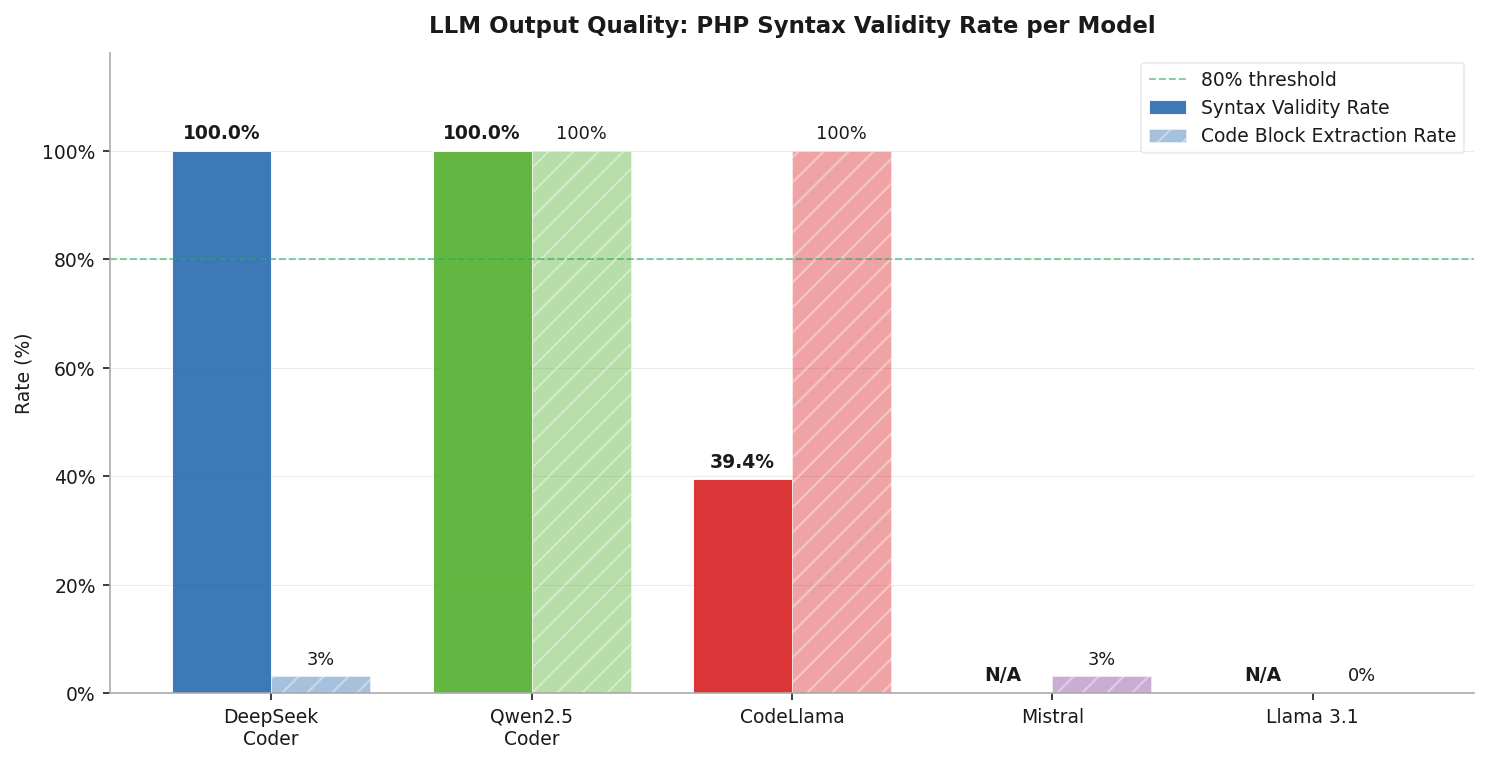
\includegraphics[width=0.77\textwidth]{contents/chapter-4/llm_quality_chart_20260427_133011.png}
    \caption{Syntax validity rate and code block extraction rate of the five LLM models in Condition B}
    \label{fig:syntax-validity-b}
\end{figure}

Qwen2.5-Coder maintained its position as the model with the best code quality: extraction rate increased from 97\% to 100\% and syntax validity remained at 100\%. CodeLlama showed partial improvement in syntax validity, from 27.3\% to 39.4\%, though still far from a reliable threshold. DeepSeek Coder experienced a decline in extraction rate from 9\% to 3\% despite its improved format compliance, indicating a trade-off between format adherence and the ability to generate code blocks. Mistral and Llama 3.1 effectively produced no usable code in Condition B.

\subsubsection{Summary Statistics}

Figure~\ref{fig:stats-table-b} summarizes the complete statistics for all five models in Condition B.

\begin{figure}[h]
    \centering
    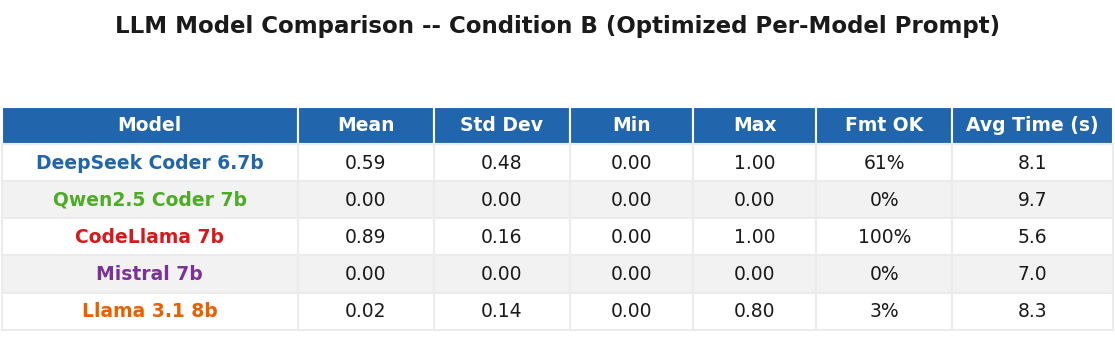
\includegraphics[width=\textwidth]{contents/chapter-4/llm_chart_20260427_140238_4_stats_tables.png}
    \caption{Complete comparison statistics for the five LLM models in Condition B}
    \label{fig:stats-table-b}
\end{figure}

DeepSeek Coder recorded the most striking increase in mean confidence, from $\bar{C}_m = 0.132$ in Condition A to $\bar{C}_m = 0.588$ in Condition B. The high variance ($\sigma_m = 0.477$) indicates that this score is unstable: some runs produced scores approaching 1.0 while others remained at 0.0. This pattern is consistent with the 61\% format compliance: only roughly two-thirds of trials actually wrote a \texttt{CONFIDENCE:} line, while the rest did not.

CodeLlama maintained a high mean confidence ($\bar{C}_m = 0.894$) with a small standard deviation ($\sigma_m = 0.162$), reflecting the same consistency as in Condition A. While this figure may appear reassuring, it must be noted that CodeLlama's syntax validity rate was only 39.4\%: the model expresses high confidence in its answers even though more than half of the code it generates fails \texttt{php -l}. This result again confirms that self-reported confidence scores cannot serve as a proxy for code quality.

Qwen2.5-Coder, Mistral, and Llama 3.1 all recorded a mean confidence of 0.000 because none of their responses wrote a \texttt{CONFIDENCE:} line in a parseable format. Specifically for Qwen2.5-Coder, the absence of a score does not reflect poor quality: the model continued to produce code with 100\% syntax validity in Condition B, the same as in Condition A. The absence of a confidence score solely reflects the model's response style of ignoring format instructions while executing its primary task well.

Overall, the same pattern from Condition A repeats: there is no reliable correlation between a high confidence score and the quality of the generated code. This reinforces the argument that for locally running small-to-medium LLMs, syntax validity rate remains the more valid evaluation metric compared to self-reported confidence scores.

% ============================================================
\subsection{Comparison of Conditions A and B}
% ============================================================

Table~\ref{tab:ab-comparison} summarizes the comparison of primary metrics between Conditions A and B for all five models.

\begin{table}[h]
\caption{Comparison of primary metrics between Conditions A and B for the five LLM models}
\vspace{0.5em}
\centering
\label{tab:ab-comparison}
\resizebox{\textwidth}{!}{%
\begin{tabular}{|l|c|c|c|c|c|c|}
\hline
\multirow{2}{*}{\textbf{Model}} &
  \multicolumn{2}{c|}{\textbf{Format Compliance}} &
  \multicolumn{2}{c|}{\textbf{Extraction Rate}} &
  \multicolumn{2}{c|}{\textbf{Syntax Validity}} \\
\cline{2-7}
 & \textbf{Cond.~A} & \textbf{Cond.~B} &
   \textbf{Cond.~A} & \textbf{Cond.~B} &
   \textbf{Cond.~A} & \textbf{Cond.~B} \\
\hline \hline
DeepSeek Coder 6.7b
  & 15\%  & \textbf{61\%} $\uparrow$
  & 9\%   & 3\% $\downarrow$
  & 100\% & 100\% \\
\hline
Qwen2.5-Coder 7b
  & 0\%   & 0\%
  & 97\%  & \textbf{100\%} $\uparrow$
  & 100\% & 100\% \\
\hline
CodeLlama 7b
  & 100\% & 100\%
  & 100\% & 100\%
  & 27\%  & \textbf{39\%} $\uparrow$ \\
\hline
Mistral 7b
  & 6\%   & 0\% $\downarrow$
  & 3\%   & 3\%
  & 0\%   & 0\% \\
\hline
Llama 3.1 8b
  & 0\%   & 3\% $\uparrow$
  & 3\%   & 0\% $\downarrow$
  & 100\% & 0\% $\downarrow$ \\
\hline
\end{tabular}%
}
\end{table}

Three main patterns can be identified from this comparison.

\textbf{First}, prompt optimization only works significantly for models that already have adequate baseline instruction-following capability. DeepSeek Coder is the only model that showed a substantial improvement in format compliance (from 15\% to 61\%), confirming that this model is sensitive to instruction complexity: it is not incapable of following the format, but was burdened by overly layered instructions in Condition A.

\textbf{Second}, applying a few-shot strategy to Mistral produced contradictory results: format compliance dropped from 6\% to 0\%. This phenomenon — where few-shot examples actually distract the model from its primary task — is consistent with findings in the literature showing that prompt engineering techniques effective for large models cannot always be directly applied to small-to-medium models \cite{akuthota2023vulnerability}.

\textbf{Third}, CodeLlama's limitation in producing syntactically valid PHP code is structural, not instructional. Although explicit instructions to verify syntax before writing code produced a partial improvement (from 27\% to 39\%), the majority of generated code still contains parse errors. This indicates that the problem is rooted in the model's internal representation of PHP 8.x syntax, not in how the instructions are formulated.

Overall, the Condition B results reinforce the conclusion from Condition A that model selection is a more determining factor than prompt strategy in the context of PHP code security analysis using locally running small-to-medium LLMs. Qwen2.5-Coder consistently produced the highest-quality code across both conditions, regardless of the prompt format provided.

% ============================================================
\subsection{Parameter Optimization for Qwen2.5-Coder (Condition C)}
% ============================================================

Having identified Qwen2.5-Coder as the model with the best code quality in Conditions A and B, Condition C evaluates whether its performance can be further improved through variations in two inference parameters: temperature and context window. This experiment uses the same input, number of runs, and prompt as Condition A; only the tested parameters differ.

Figure~\ref{fig:kondisi-c} shows the comparison of the three primary metrics across all parameter variations.

\begin{figure}[h]
    \centering
    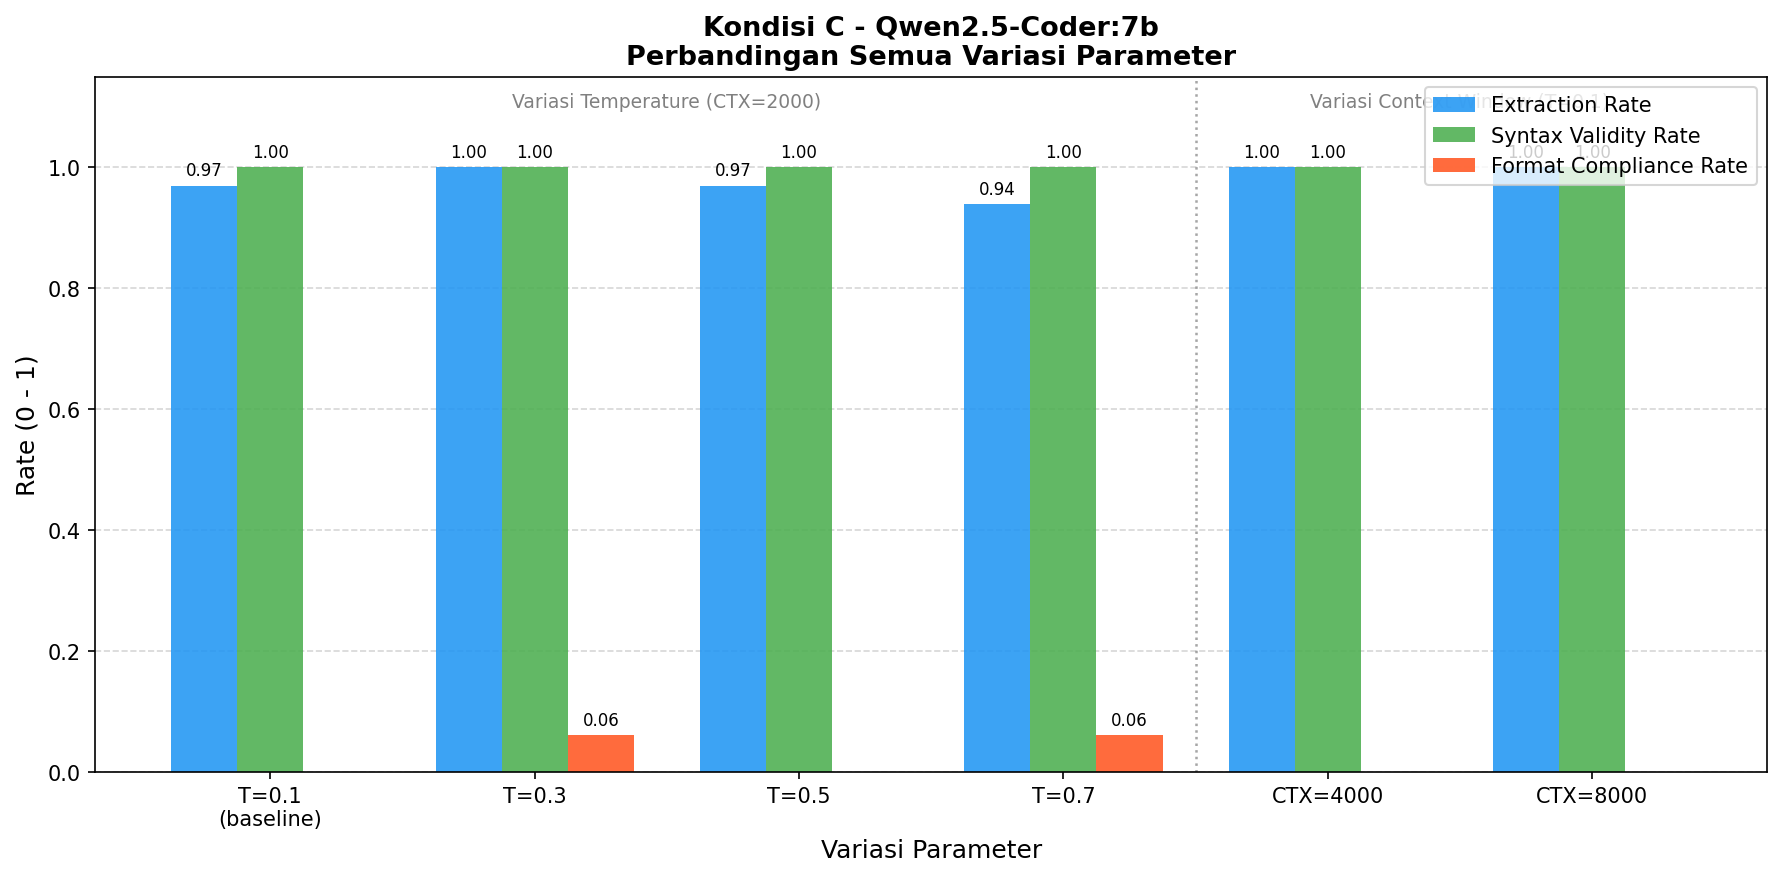
\includegraphics[width=1\textwidth]{contents/chapter-4/llm_chart_kondisi_c_parameter_comparison.png}
    \caption{Comparison of Qwen2.5-Coder metrics across temperature and context window variations (Condition C)}
    \label{fig:kondisi-c}
\end{figure}

\subsubsection{Effect of Temperature}

The temperature value T=0.1 was not retested in Condition C because it was already used as the baseline in Condition A; Condition C only tests values T=0.3 through T=0.7 to observe the effect of increasing temperature on model performance.

In the temperature variation, syntax validity rate remained at 100\% across all tested values (0.3 through 0.7). This data shows that Qwen2.5-Coder's ability to produce syntactically valid PHP code does not degrade even when temperature is increased substantially.

Extraction rate declined slightly as temperature increased: from 100\% at T=0.3 to 94\% at T=0.7. This is consistent with the theoretical expectation that higher temperatures increase response variability, causing a small fraction of responses to no longer contain an extractable code block.

Format compliance showed a non-monotonic pattern: it appeared at T=0.3 (6\%) and T=0.7 (6\%), but returned to 0\% at T=0.5. This inconsistent appearance of format compliance indicates that adherence to format in Qwen2.5-Coder is more influenced by stochastic variability than by systematic temperature changes.

\subsubsection{Effect of Context Window}

In the context window variation, both CTX=4000 and CTX=8000 produced extraction rates and syntax validity rates of 100\%, slightly above the CTX=2000 baseline which had a 97\% extraction rate. Format compliance remained at 0\% in both variations.

The increase in extraction rate from 97\% to 100\% under larger context sizes indicates that with more complete code information, the model more consistently generates a code block in each response. However, this improvement is marginal and does not alter the model's fundamental characteristics.

\subsubsection{Implications of Condition C}

Condition C shows that the characteristics of Qwen2.5-Coder are more determined by its model architecture than by parameter configuration. The quality of the generated code is highly stable across all tested parameter variations. In practice, this means operators do not need to perform extensive parameter tuning to obtain quality output from this model. The default configuration (T=0.1, CTX=2000) already delivers near-optimal results, while increasing the context window to 4000 or 8000 characters can provide a slight additional benefit for longer code files.

% ============================================================
\subsection{Composer Dependency Analysis}
% ============================================================

The \texttt{composer\_analyzer.py} module reads the \texttt{composer.json} file at the FT UGM repository root and checks the PHP 8.x compatibility of each dependency using data from Packagist. Five dependencies were identified, with results as shown in Table~\ref{tab:composer-ft}.

\begin{table}[h]
\caption{PHP 8.x compatibility status of FT UGM composer dependencies}
\vspace{0.5em}
\centering
\label{tab:composer-ft}
\begin{tabularx}{\textwidth}{|l|l|X|}
\hline
\textbf{Package} & \textbf{Version} & \textbf{Status} \\
\hline \hline
\texttt{vlucas/phpdotenv} & \texttt{\^{}5.4} & \texttt{SAFE} \\
\hline
\texttt{phpoffice/phpspreadsheet} & \texttt{\^{}1.12} & \texttt{SAFE} \\
\hline
\texttt{firebase/php-jwt} & \texttt{\^{}6.10} & \texttt{SAFE} \\
\hline
\texttt{ngekoding/google-login} & \texttt{\^{}1.0} & \texttt{MANUAL REVIEW} \\
\hline
\texttt{chriskacerguis/codeigniter-restserver} & \texttt{\^{}3.1} & \texttt{MANUAL REVIEW} \\
\hline
\end{tabularx}
\end{table}

Three of the five dependencies (\texttt{phpdotenv}, \texttt{phpspreadsheet}, \texttt{firebase/\allowbreak php-jwt}) have a \texttt{SAFE} status, meaning the versions configured in \texttt{composer.json} already declaratively support PHP 8.x. The other two dependencies have a \texttt{MANUAL REVIEW} status: \texttt{ngekoding/\allowbreak google-login} is a package with low maintenance activity whose PHP 8.x compatibility cannot be verified automatically, while \texttt{chriskacerguis/\allowbreak codeigniter-restserver} is a third-party extension for CodeIgniter 3.x that is known to lack official PHP 8.x support and must be replaced or updated manually before deployment to a PHP 8.3 environment.

% ============================================================
\subsection{Conversion Accuracy Validation}
% ============================================================

Accuracy validation was conducted through two approaches to objectively measure the quality of Rector's conversion output on the FT UGM dataset. Given that both datasets use the CodeIgniter 3 framework with similar code characteristics, these validation results serve as a representative measure of Rector's conversion accuracy for both case studies.

\subsubsection{Pipeline-Level Metrics}

Figure~\ref{fig:validation-metrics} shows the two accuracy metrics measured directly from the pipeline output across all 241 converted files, along with the execution duration profile.

\begin{figure}[h]
    \centering
    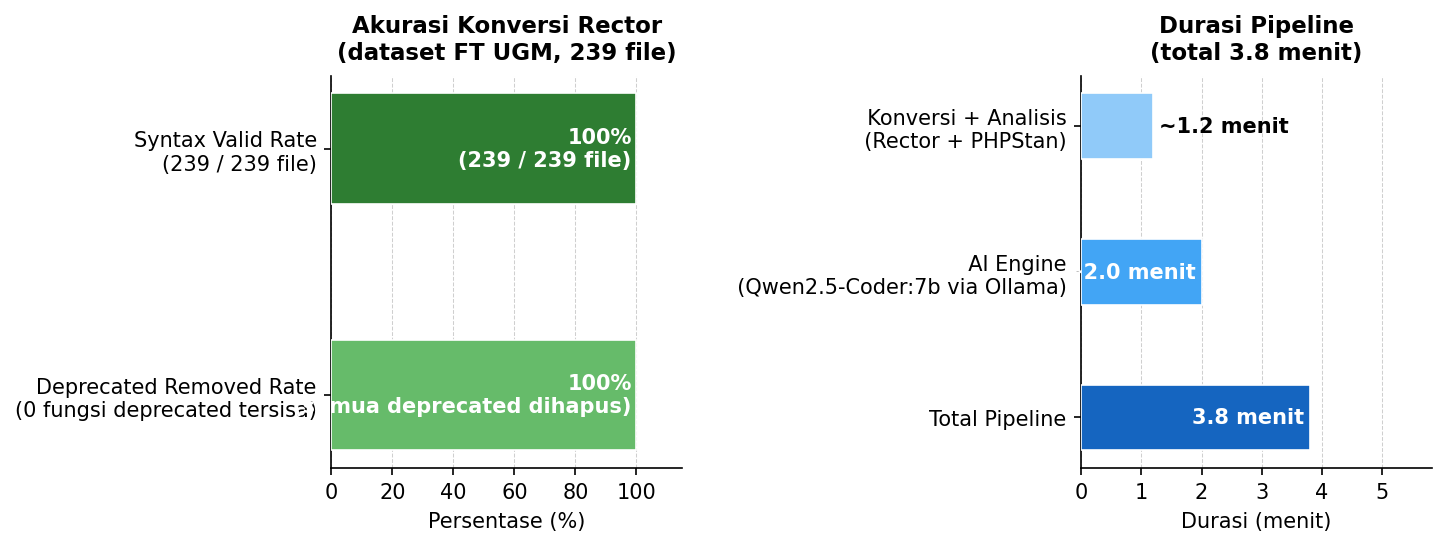
\includegraphics[width=\textwidth]{contents/chapter-4/validation/validation_metrics_qwen.png}
    \caption{Rector conversion accuracy metrics and pipeline execution duration on the FT UGM dataset}
    \label{fig:validation-metrics}
\end{figure}

First, the syntax validity rate was measured by running \texttt{php -l} against all files in the \texttt{output/} directory. The result was 241 out of 241 files passing with no parse errors (100\%). This means not a single file suffered syntactic corruption from the Rector conversion process.

Second, the deprecated removal rate was measured by comparing the Semgrep pre-scan and post-scan findings specifically for the deprecated function category. The post-scan result shows 0 deprecated functions remaining, meaning all deprecated code patterns detected by Semgrep were successfully removed or transformed by Rector (100\%).

In terms of duration, the total pipeline execution time is approximately 3.8 minutes using Qwen2.5-Coder 7b via Ollama as the AI Engine. This duration does not include the multi-model comparison experiments (Conditions A through C), which are separate evaluation procedures. The Rector conversion and PHPStan analysis stages together dominate the execution time.

\subsubsection{10\% Sampling Validation}

To measure how closely Rector's conversion output matches an ideal manual conversion, a sampling-based validation was performed on 10\% of the total valid files. A total of 24 files were selected at random (seed=42) from all valid files that passed the \texttt{php -l} check using the \texttt{accuracy\_validator.py} module, representing 10\% of the total valid file population.

Figure~\ref{fig:validation-coverage} shows the distribution of coverage across the 24 sampled files.

\begin{figure}[h]
    \centering
    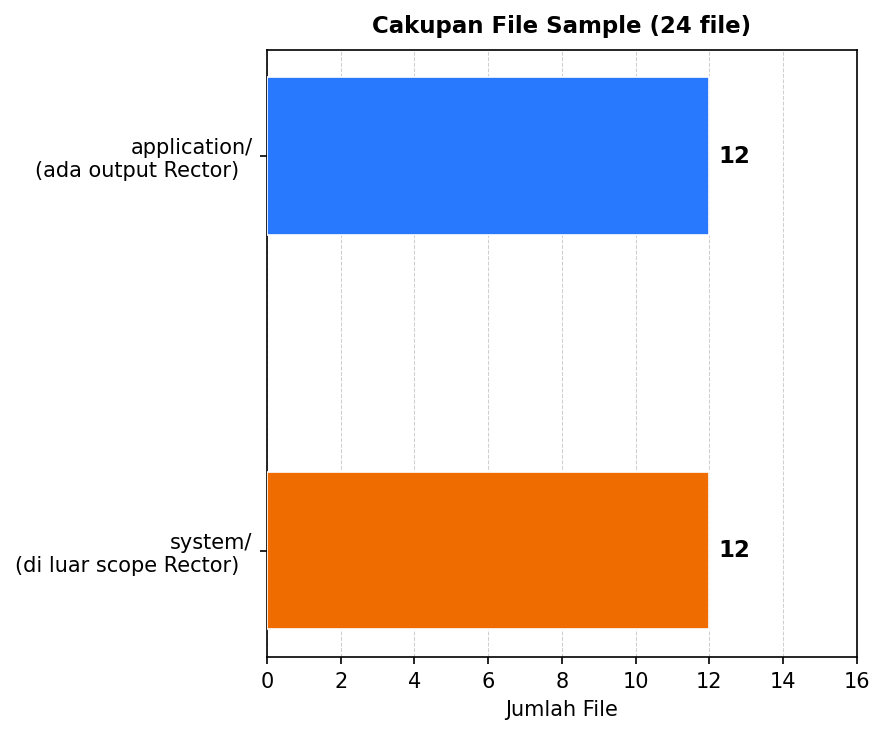
\includegraphics[width=0.6\textwidth]{contents/chapter-4/validation/validation_accuracy_qwen_3_coverage.png}
    \caption{Coverage distribution of the 10\% validation sample files by source directory}
    \label{fig:validation-coverage}
\end{figure}

Of the 24 sampled files, 12 come from the \texttt{application/} directory (application code processed by Rector) and 12 from the \texttt{system/} directory (framework code that was also converted). Since the comparison is made between Rector's output and a reference conversion prepared manually by the researcher with the assistance of an enterprise LLM as a proxy for ideal conversion, only the 12 files from \texttt{application/} have a corresponding Rector output to compare against. Files from \texttt{system/} are retained in the sample for transparency of the sampling procedure.

Figure~\ref{fig:validation-sampling} shows the comparison between Rector's output and the LLM reference on those 12 files.

\begin{figure}[h]
    \centering
    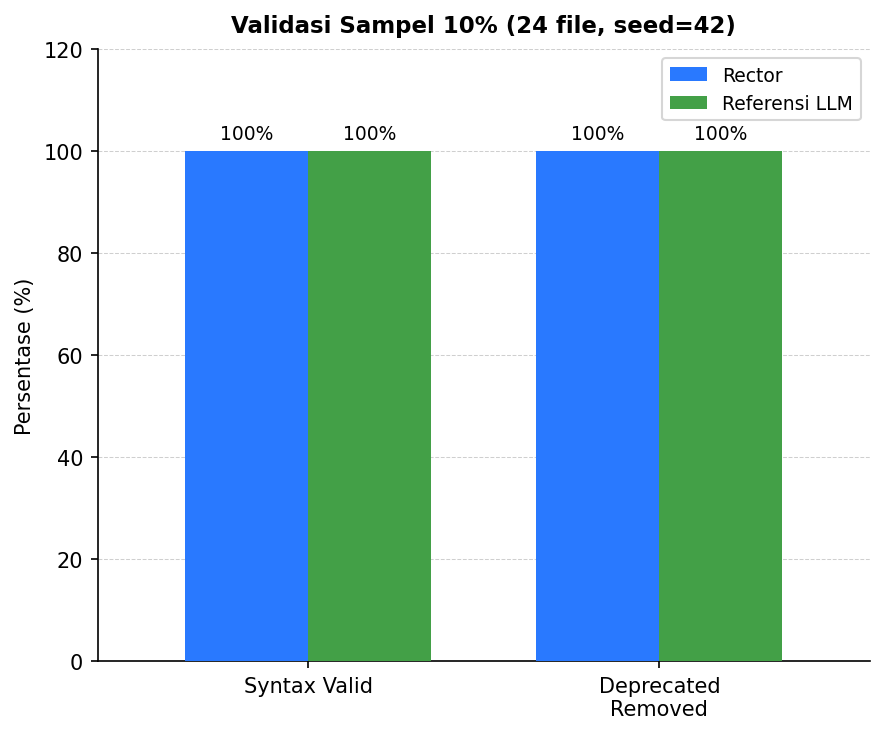
\includegraphics[width=0.6\textwidth]{contents/chapter-4/validation/validation_accuracy_qwen_1_sampling.png}
    \caption{Comparison of validation metrics between Rector output and LLM reference for 12 sample files from \texttt{application/}}
    \label{fig:validation-sampling}
\end{figure}

On both binary metrics, the Rector output and the LLM reference achieved identical results: 100\% syntax validity and 100\% deprecated removal. This confirms that Rector's conversion produces code equivalent to manual conversion in terms of syntactic correctness and removal of deprecated patterns.

Figure~\ref{fig:validation-similarity} shows the distribution of similarity scores between Rector's output and the LLM reference.

\begin{figure}[h]
    \centering
    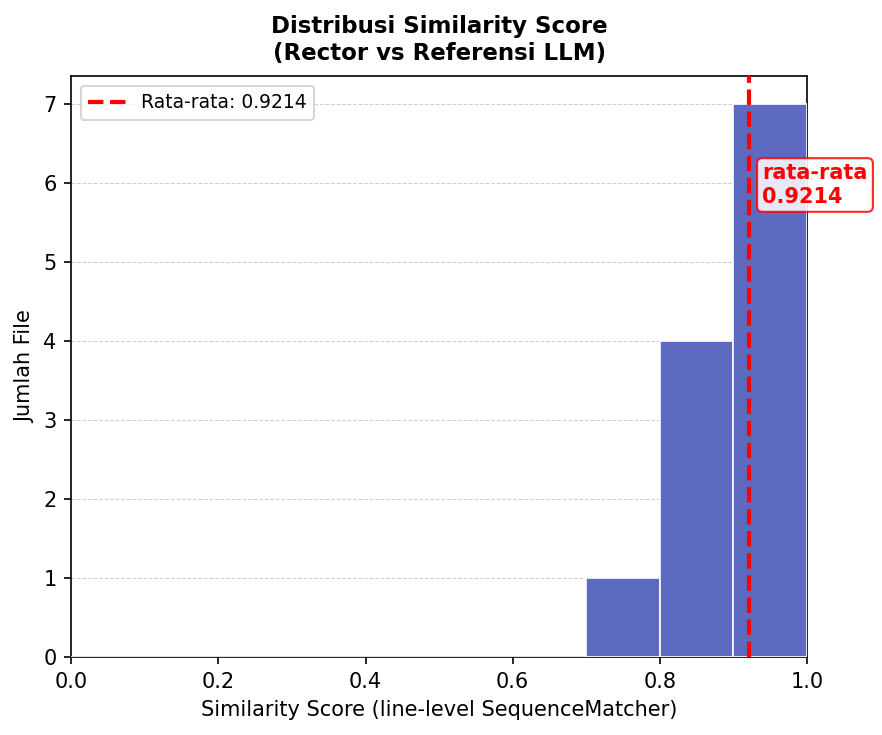
\includegraphics[width=0.65\textwidth]{contents/chapter-4/validation/validation_accuracy_qwen_2_similarity.png}
    \caption{Distribution of similarity scores between Rector output and LLM reference for 12 sample files (line-level SequenceMatcher)}
    \label{fig:validation-similarity}
\end{figure}

The similarity score is computed using a line-level SequenceMatcher that measures the proportion of identical lines between two versions of the code. The mean similarity score is 0.9214, with the distribution concentrated in the 0.90--1.00 range (11 of 12 files). One file falls in the 0.70--0.80 range, reflecting a difference in writing style between automatic AST transformation and manual conversion, not an indication of a conversion error.

A score of 0.9214 indicates a high degree of agreement between the automated AST-based approach (Rector) and the manual LLM-based approach. The remaining differences generally consist of cosmetic variations such as whitespace, attribute ordering, or coding style that do not affect the functional correctness of the code. Because both datasets use the CodeIgniter 3.x framework with similar code characteristics, these validation results also apply to the CBT DTI UGM case study.

% ============================================================
\subsection{Discussion and Limitations}
% ============================================================

\subsubsection{Dataset Limitations}

The dataset used consists of a single CodeIgniter 3.x application from FT UGM. Of the 245 files, 237 are classified as \textit{unknown} by Rector because they are CodeIgniter framework files that contain no patterns requiring transformation. This limits the generalizability of the research results to other types of PHP applications, particularly those that do not use a framework or that use a different framework.

From the perspective of the LLM experiment input, 10 of the 11 findings are SSRF vulnerabilities arising from a single repeated code pattern in \texttt{Output.php}. This input homogeneity means the comparison experiment fundamentally tests model responses to two vulnerability types with limited variation. The comparison results should be interpreted within the context of this limitation.

\subsubsection{PHP 8.4 and PHP 8.5 Compatibility Limitations}

Additional experiments were conducted to test the pipeline with a PHP 8.5 target against the CBT DTI UGM dataset. The results revealed two fundamental problems that constrain automated application to this version.

First, Rector introduced syntax errors in several core CodeIgniter 3.x files in the \texttt{system/} directory, specifically \texttt{CodeIgniter.php}, \texttt{Output.php}, and \texttt{Security.php}, because the PHP 8.5 ruleset applies transformations incompatible with legacy framework code patterns. Second, as a result of the corrupted \texttt{system/} files after conversion, PHPStan could not resolve CodeIgniter parent classes such as \texttt{CI\_Controller} and \texttt{CI\_Model}, producing thousands of cascading false-positive \textit{unknown class} errors. The total of 6,137 PHPStan errors generated is not representative of the actual application code quality.

The primary cause of these failures is not solely CodeIgniter 3's incompatibility with PHP 8.5. It is more attributable to the \texttt{UP\_TO\_PHP\_85} ruleset in Rector, which is still experimental and therefore applies overly aggressive transformations to legacy framework code.

The most viable path toward PHP 8.5 is to upgrade the framework to CodeIgniter 4 or another modern framework that natively supports PHP 8.x — a process that goes beyond the scope of automated version migration and is essentially an application rewrite. PHP 8.3 is therefore established as the target version in this research as the option achievable through automation for CodeIgniter 3.x-based applications.

\subsubsection{Technical Pipeline Limitations}
\label{sec:keterbatasan}

The AI Engine only processes findings with priority levels 1 through 5 and limits the code snippet sent to the model to the first 2,000 characters. For longer PHP files, the context received by the model is truncated, so remediation suggestions may not take the full function logic into account. As seen in the Qwen2.5-Coder response example, a model can make correct inferences about the code context with limited information, but this cannot always be guaranteed.

Furthermore, validation using \texttt{php -l} only checks syntactic correctness, not semantic correctness. Code that passes \texttt{php -l} may still contain unaddressed vulnerabilities or logic that is not equivalent to the original code. Functional testing of AI-remediated code is outside the scope of this research.

\subsubsection{Interpretation of Confidence Scores}

There is no clear correlation between the confidence scores reported by the models and the quality of the generated code, in either Condition A or Condition B. CodeLlama reported an average confidence of over 90\% in both conditions, yet the majority of the code it produced was syntactically invalid. Qwen2.5-Coder reported no score at all yet produced near-consistently high-quality code. These findings are consistent with the literature showing that small-scale LLMs are generally poorly calibrated in assessing their own output \cite{akuthota2023vulnerability}\cite{li2025iris}.

Of the three metrics measured — FCR, extraction rate, and SVR — only SVR consistently reflects the practical utility of a model in this context.

% ============================================================
\section{Case Study 2: CBT System, DTI UGM}
% ============================================================

% ------------------------------------------------------------
\subsection{Dataset Description}
% ------------------------------------------------------------

The second case study uses the source code of the Computer-Based Test (CBT) application belonging to the Directorate of Information Technology (DTI), Universitas Gadjah Mada. The application is built on the CodeIgniter 3 framework with a PHP 5.x/7.x codebase. The pipeline was run against the entire repository directory in full scope, covering the \texttt{application/} directory for custom application code as well as the \texttt{system/} directory for framework code, consistent with the approach applied in the FT UGM case study. The only exceptions are the \texttt{libraries/} and \texttt{tcpdf/} subdirectories, which caused memory crashes during the analysis process. The total number of PHP files processed is 326.

Because there is no \texttt{composer.json} file at the application level, the dependency analysis step was automatically skipped. Third-party components such as the TCPDF library are included directly as directories within the repository and have been excluded from the pipeline analysis.

% ------------------------------------------------------------
\subsection{Rector Conversion Results}
% ------------------------------------------------------------

Rector was run against 326 PHP files with a target version of PHP 8.3. Of these, 299 files were successfully converted, 25 were skipped, and 2 failed to process. The overall conversion rate ($CR = 91.7\%$) is shown in Figure~\ref{fig:rector-bar-dti}.

\newpage
\begin{figure}[h]
    \centering
    
\includegraphics[width=0.8\textwidth]{contents/chapter-4/dti/pipeline_chart_cbt_qwen_2a_rector_bar.png}
    \caption{Summary of Rector conversion results for 326 PHP files from the CBT DTI UGM dataset}
    \label{fig:rector-bar-dti}
\end{figure}

The lower conversion rate compared to the FT UGM case study (91.7\% vs 97.6\%) is attributable to the larger proportion of skipped files: 25 of 326 files (7.7\%) required no transformation because their code was already compatible with the PHP 8.3 target or contained no patterns covered by Rector's rulesets. Skipped files are not failures; they already satisfy the PHP 8.3 requirements without modification.

All files in the \texttt{output/} directory were tested for syntax validity using \texttt{php -l} and no parse errors were found, giving a post-conversion syntax validity rate of 100\%.

\subsubsection{Files That Failed Conversion}

Both files that failed conversion — \texttt{captcha\_helper.php} and \texttt{form\_helper.php} — encountered the same internal error as in the FT UGM dataset: the \texttt{FiberNodeScopeResolver} bug in the version of Rector used, not originating from the CBT DTI source code. The code characteristics that trigger this bug are identical: \texttt{captcha\_helper.php} contains a branch with different return types, while \texttt{form\_helper.php} has numerous conditional function definitions wrapped in \texttt{if (!function\_exists(\ldots))} constructs. Both files are copied to the \texttt{output/} directory as the original code so that the conversion process retains all data.

% ------------------------------------------------------------
\subsection{Semgrep Security Scan Results}
% ------------------------------------------------------------

\subsubsection{Pre-Scan: Original Code Security Baseline}

The Semgrep scan against 326 PHP files in the \texttt{input/} directory produced 11 findings, comprising 1 SQL Injection vulnerability and 10 SSRF (Server-Side Request Forgery) vulnerabilities, as shown in Figures~\ref{fig:semgrep-severity-dti} and~\ref{fig:semgrep-vulntype-dti}.

\begin{figure}[h]
    \centering
    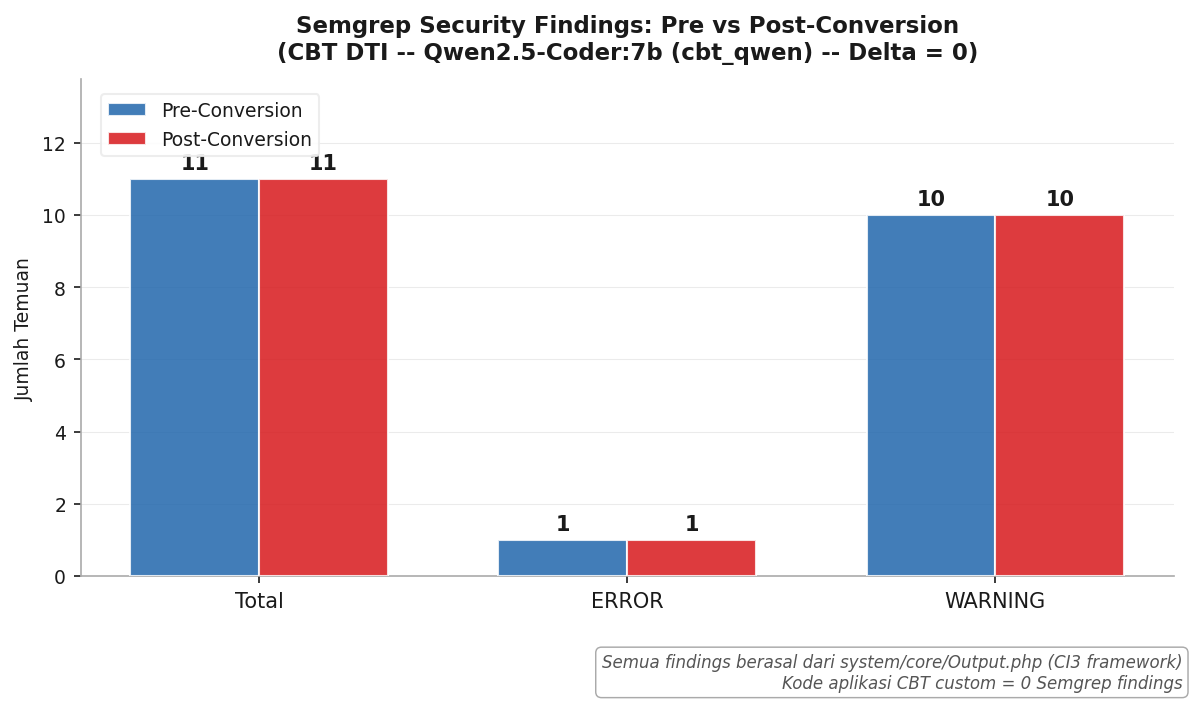
\includegraphics[width=0.8\textwidth]{contents/chapter-4/dti/pipeline_chart_cbt_qwen_1a_semgrep_severity.png}
    \caption{Semgrep pre-scan vs post-scan findings by severity level on the CBT DTI UGM dataset}
    \label{fig:semgrep-severity-dti}
\end{figure}

\begin{figure}[h]
    \centering
    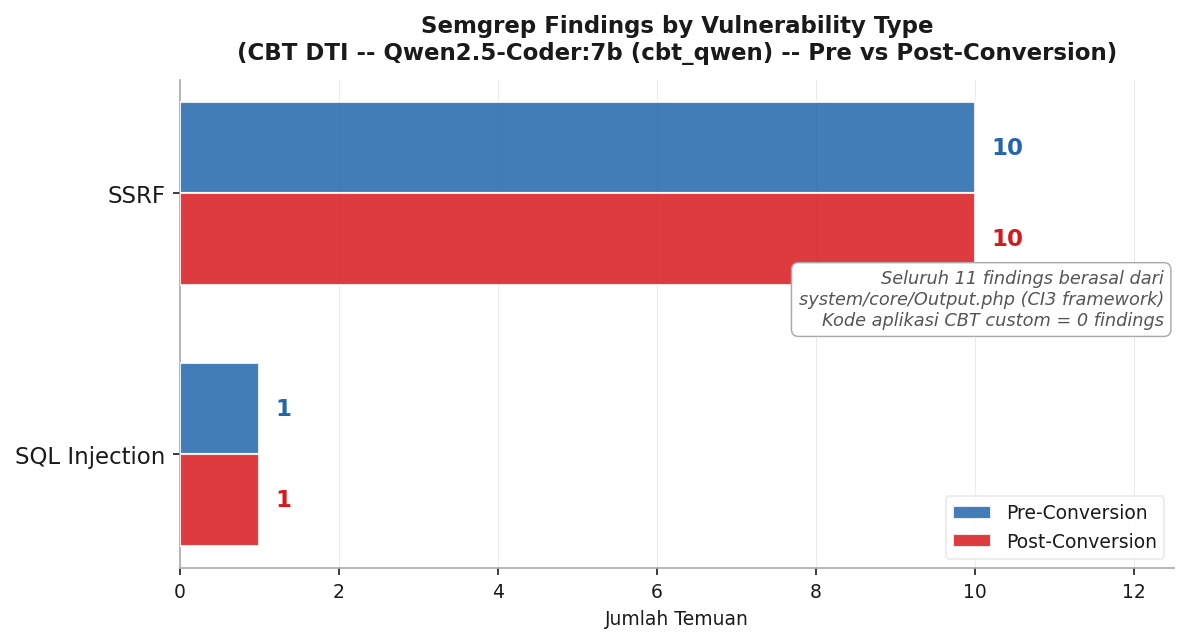
\includegraphics[width=0.85\textwidth]{contents/chapter-4/dti/pipeline_chart_cbt_qwen_1b_semgrep_vulntype.png}
    \caption{Semgrep pre-scan vs post-scan findings by vulnerability type on the CBT DTI UGM dataset}
    \label{fig:semgrep-vulntype-dti}
\end{figure}

All 11 findings are localized to a single file: \texttt{system/core/\allowbreak Output.php}, a core component of the CodeIgniter 3 framework. The finding pattern is identical to that found in the FT UGM dataset: a SQL Injection vulnerability at line 768 due to use of \texttt{\$\_SERVER['QUERY\_STRING']} without sanitization in cache path construction, and 10 SSRF vulnerabilities from the use of user-input-derived filenames in file system operations. The custom CBT DTI application code outside the \texttt{system/} directory contains no Semgrep findings.

\subsubsection{Post-Scan and AI Engine}

The Semgrep scan against the \texttt{output/} directory after conversion produced a finding count identical to the pre-scan: 11 findings ($\Delta F = F_{post} - F_{pre} = 0$). The distribution of vulnerability types also remained the same, all in \texttt{system/core/\allowbreak Output.php}. This confirms that Rector's conversion introduced no new vulnerabilities nor removed any existing ones, consistent with the characteristics of AST-based transformation that modifies syntax without altering program logic.

Because there were 11 Semgrep findings, the AI Engine module was automatically activated by the pipeline. The \textit{qwen2.5-coder:7b} model via Ollama processed all 11 findings and generated remediation suggestions with an average confidence of 26\%. The model was selected based on the comparison experiment results from the FT UGM case study, which identified Qwen2.5-Coder as the model with the best code quality. The one exception was the SQL Injection finding in \texttt{Output.php} at line 768, which received a confidence of 0\%, because the code snippet sent to the model did not include enough context to analyze the internal framework construction. All remediation suggestions from the AI Engine are informational and require manual review before being applied, as all findings originate from framework code that should not be modified directly.

% ------------------------------------------------------------
\subsection{PHPStan Validation Results}
% ------------------------------------------------------------

PHPStan level 5 was run against the converted code in the \texttt{output/} directory targeting PHP 8.3. The result was 2,354 findings. Of these, 318 are false positives from the CodeIgniter 3 framework that arise because PHPStan cannot trace magic properties and helper functions injected dynamically, consistent with the 354 CI3 noise items identified in the FT UGM dataset. The distribution of findings by ISO/IEC 27001:2022 control is shown in Figure~\ref{fig:phpstan-iso-dti}.

\begin{figure}[h]
    \centering
    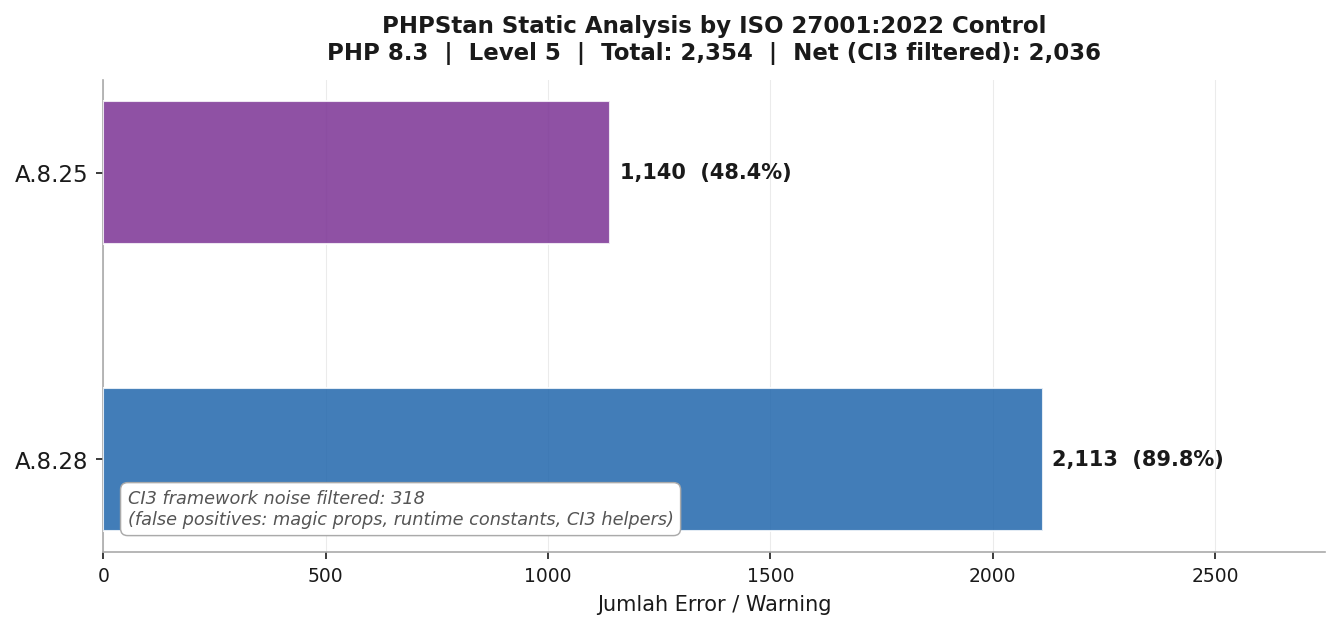
\includegraphics[width=0.8\textwidth]{contents/chapter-4/dti/pipeline_chart_cbt_qwen_3a_phpstan_bar.png}
    \caption{Distribution of PHPStan findings by ISO/IEC 27001:2022 Annex A control on the CBT DTI UGM dataset}
    \label{fig:phpstan-iso-dti}
\end{figure}

As in the FT UGM case study, the majority of PHPStan findings in the CBT DTI dataset originate from PHPStan's limitations in understanding the CodeIgniter 3.x architecture. PHPStan cannot trace two categories of elements dynamically injected by the framework at runtime: (1) magic properties such as \texttt{\$this->db} and \texttt{\$this->load} originating from \texttt{CI\_Controller} and \texttt{CI\_Model}, and (2) helper functions such as \texttt{base\_url()}, \texttt{redirect()}, and \texttt{form\_open()} that are loaded dynamically. Because the CodeIgniter \texttt{system/} directory is analyzed together with the application code, PHPStan generates a large number of \textit{undefined} reports for these elements, which are framework false positives.

The PHPStan error distribution pattern in the CBT DTI dataset shows a high concentration in control A.8.28 (Secure Coding) with 2,113 findings (89.8\% of the total), while A.8.25 (Secure Development Lifecycle) recorded 1,140 findings (48.4\%). As in the first case study, the high PHPStan numbers reflect accumulated technical debt that existed prior to migration, not errors introduced by the conversion process.

% ------------------------------------------------------------
\subsection{ISO/IEC 27001:2022 Compliance Status}
% ------------------------------------------------------------

Based on the mapping performed by \texttt{iso\_mapper.py}, the compliance status for the six mapped ISO/IEC 27001:2022 controls is shown in Table~\ref{tab:iso-status-dti}.

\newpage
\begin{longtable}{|l|>{\raggedright\arraybackslash}p{2.5cm}|p{6cm}|p{3cm}|}
\caption{ISO/IEC 27001:2022 compliance status from the pipeline on the CBT DTI UGM dataset}
\label{tab:iso-status-dti} \\
\hline
\textbf{Control} & \textbf{Title} & \textbf{Assessment Basis} & \textbf{Status} \\
\hline \hline
\endfirsthead

\multicolumn{4}{l}{\textit{(continued from Table \ref{tab:iso-status-dti})}} \\
\hline
\textbf{Control} & \textbf{Title} & \textbf{Assessment Basis} & \textbf{Status} \\
\hline \hline
\endhead

\hline
\multicolumn{4}{r}{\textit{(continued on next page)}} \\
\endfoot

\hline
\endlastfoot

A.5.17 & Authentication Information &
No hardcoded credentials findings &
\texttt{COMPLIANT} \\
\hline

A.8.24 & Use of Cryptography &
No findings of \texttt{md5()}/\texttt{sha1()} used for password storage &
\texttt{COMPLIANT} \\
\hline

A.8.25 & Secure Development Lifecycle &
1,140 PHPStan findings (majority CI3 false positives) &
{\footnotesize\ttfamily NON\_COMPLIANT} \\
\hline

A.8.26 & Application Security Requirements &
1 SQL Injection finding from Semgrep (\texttt{Output.php}, CI3 framework) &
{\footnotesize \texttt{NON\_COMPLIANT}} \\
\hline

A.8.28 & Secure Coding &
2,113 PHPStan findings and active Semgrep findings &
{\footnotesize \texttt{NON\_COMPLIANT}} \\
\hline

A.8.29 & Security Testing in Development &
10 open SSRF findings from Semgrep &
{\footnotesize \texttt{NON\_COMPLIANT}} \\
\end{longtable}

The \texttt{NON\_COMPLIANT} status for A.8.26 and A.8.29 originates from \texttt{system/core/\allowbreak Output.php} of the CodeIgniter 3 framework, not from the custom CBT DTI application code. This result is consistent with the full-scope analysis approach applied in both case studies.

% ------------------------------------------------------------
\subsection{Composer Dependency Analysis}
% ------------------------------------------------------------

The CBT DTI UGM application has no \texttt{composer.json} file at the application level. Third-party components such as the TCPDF library are included directly as directories within the repository and have been excluded from the pipeline analysis. The \texttt{composer\_analyzer.py} module therefore produces no output for this case study, and the dependency analysis step is automatically skipped.

% ============================================================
\section{Comparison of Both Case Studies}
% ============================================================

This section compares the pipeline implementation results from both case studies side by side to identify consistent patterns and significant differences.

% ------------------------------------------------------------
\subsection{Comparison of Semgrep Security Findings}
% ------------------------------------------------------------

Figure~\ref{fig:comparison-semgrep} shows the comparison of Semgrep pre-scan findings by vulnerability type across both datasets.

\begin{figure}[h]
    \centering
    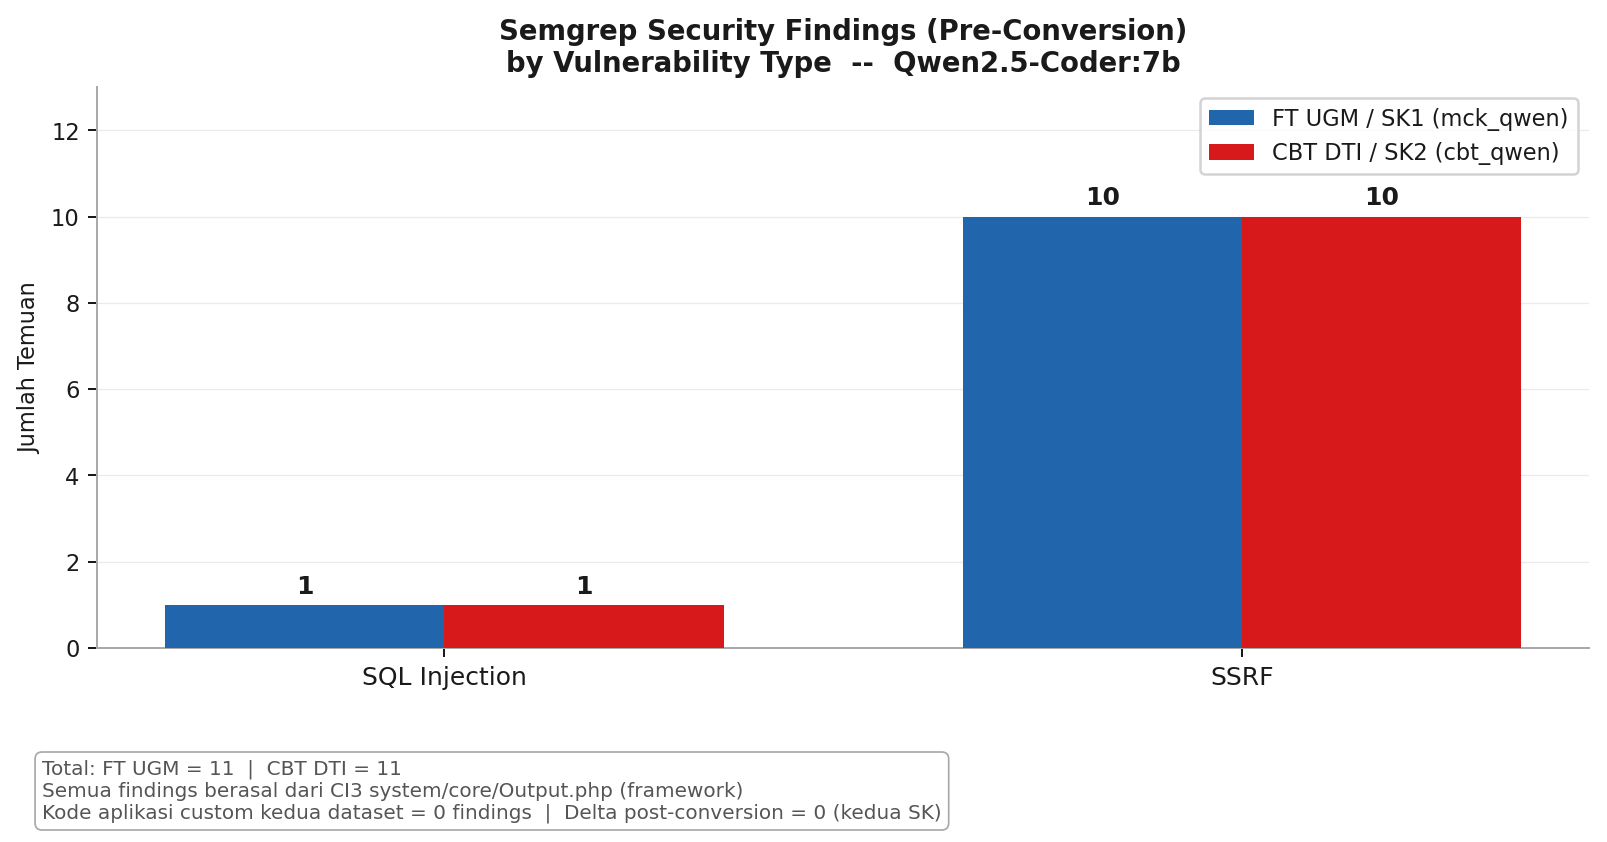
\includegraphics[width=0.95\textwidth]{contents/chapter-4/comparison/comparison_qwen_1_semgrep_findings.png}
    \caption{Comparison of Semgrep pre-scan findings by vulnerability type across both case studies}
    \label{fig:comparison-semgrep}
\end{figure}

The FT UGM and CBT DTI datasets each produced 11 Semgrep pre-scan findings, all localized to \texttt{system/core/Output.php}, a core component of CodeIgniter 3. The finding pattern is identical: 1 SQL Injection and 10 SSRF in both datasets. This pattern confirms that both applications use the same version of CodeIgniter 3 with unmodified framework code. The custom application code in both datasets produced no Semgrep findings.

In both case studies, $\Delta F = 0$ confirms that Rector's conversion neither introduced nor removed any vulnerabilities. The existing findings require remediation at the framework code level, which lies outside the scope of automatic syntactic transformation.

% ------------------------------------------------------------
\subsection{Comparison of Rector Conversion Rates}
% ------------------------------------------------------------

Figure~\ref{fig:comparison-rector} shows the comparison of Rector conversion results across both datasets.

\begin{figure}[h]
    \centering
    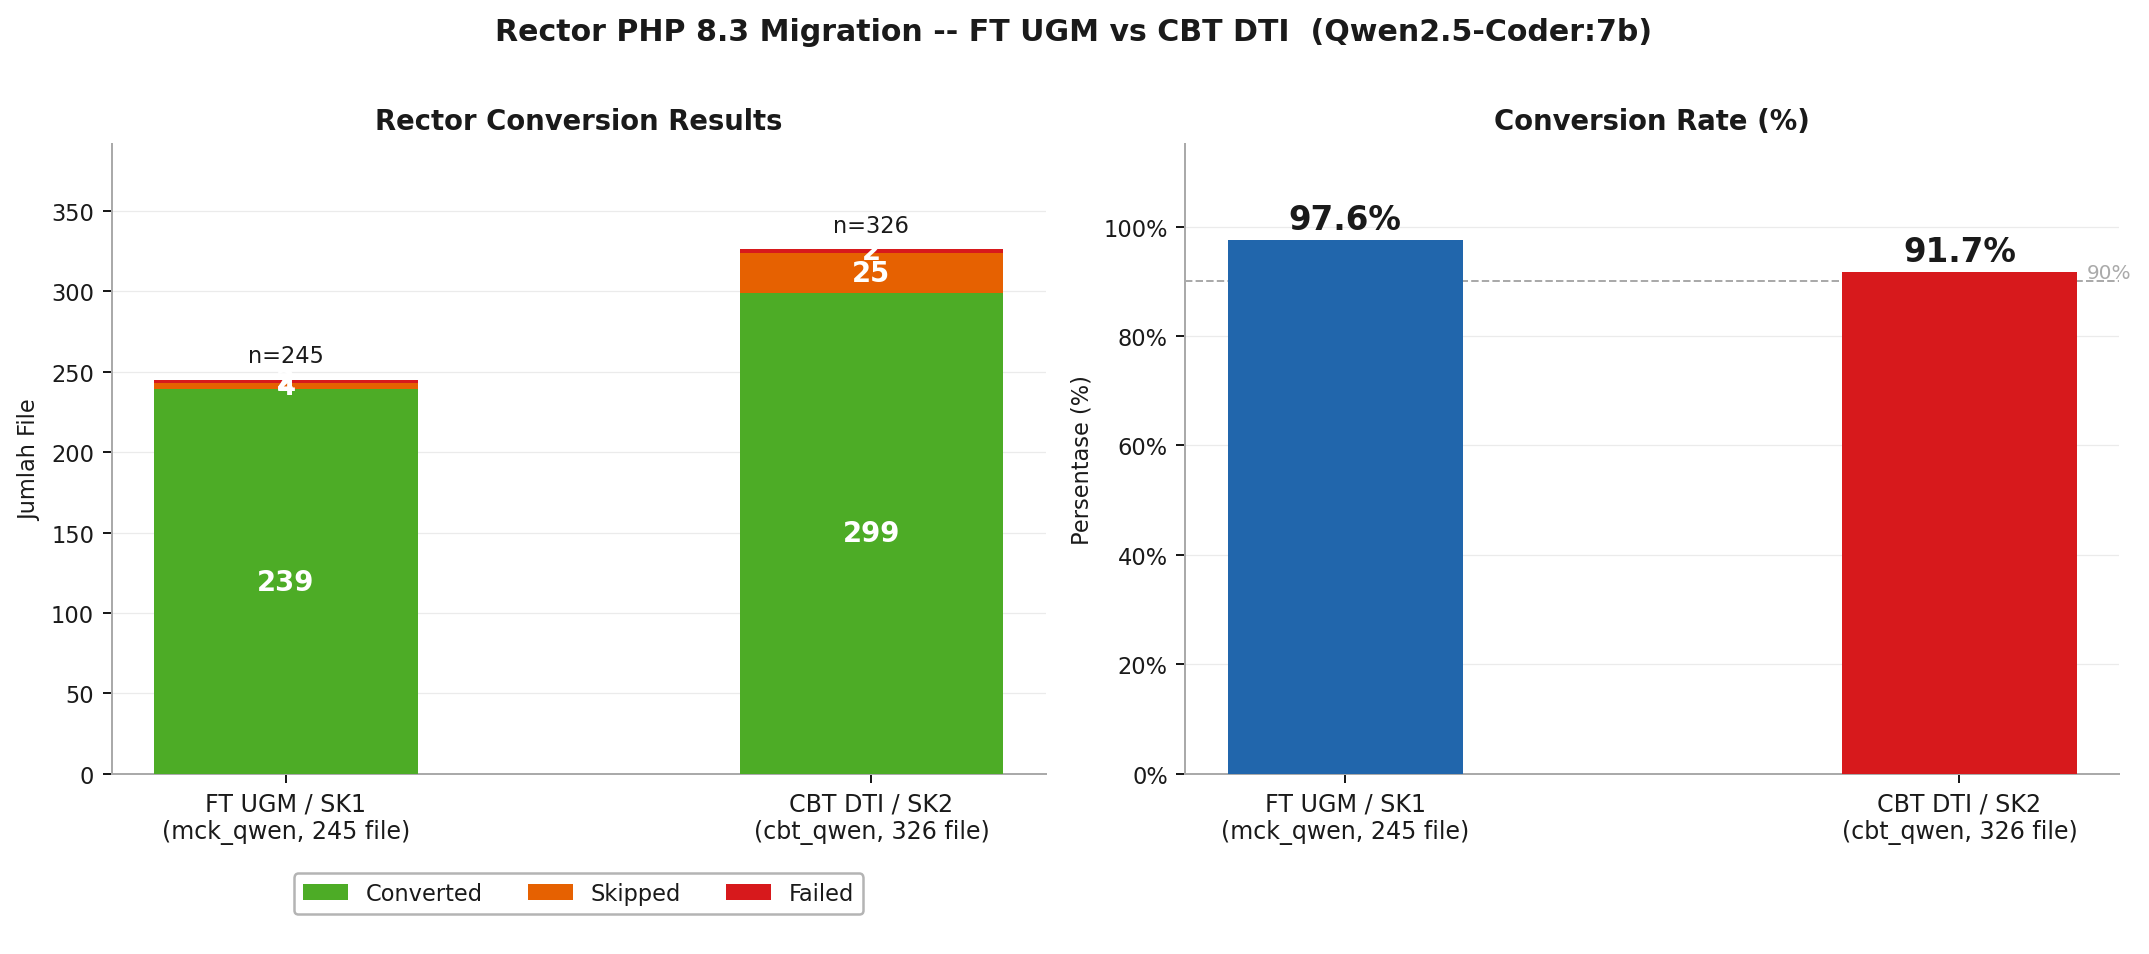
\includegraphics[width=1.0\textwidth]{contents/chapter-4/comparison/comparison_qwen_2_rector_conversion.png}
    \caption{Comparison of Rector conversion results across both case studies}
    \label{fig:comparison-rector}
\end{figure}

FT UGM recorded a conversion rate of 97.6\% (239/245) while CBT DTI recorded 91.7\% (299/326). The 5.9 percentage point difference is primarily attributable to the proportion of skipped files: CBT DTI had 25 skipped files (7.7\%) compared to 4 in FT UGM (1.6\%). Both datasets experienced failures in the same 2 files (\texttt{captcha\_helper.php} and \texttt{form\_helper.php}) due to the \texttt{FiberNodeScopeResolver} bug in Rector, confirming that this failure is systemic to the version of Rector used and not specific to either dataset. Post-conversion syntax validity reached 100\% in both case studies.

% ------------------------------------------------------------
\subsection{Comparison of PHPStan Findings}
% ------------------------------------------------------------

Figure~\ref{fig:comparison-phpstan} shows the comparison of PHPStan error distributions by ISO/IEC 27001:2022 control across both datasets.

\begin{figure}[h]
    \centering
    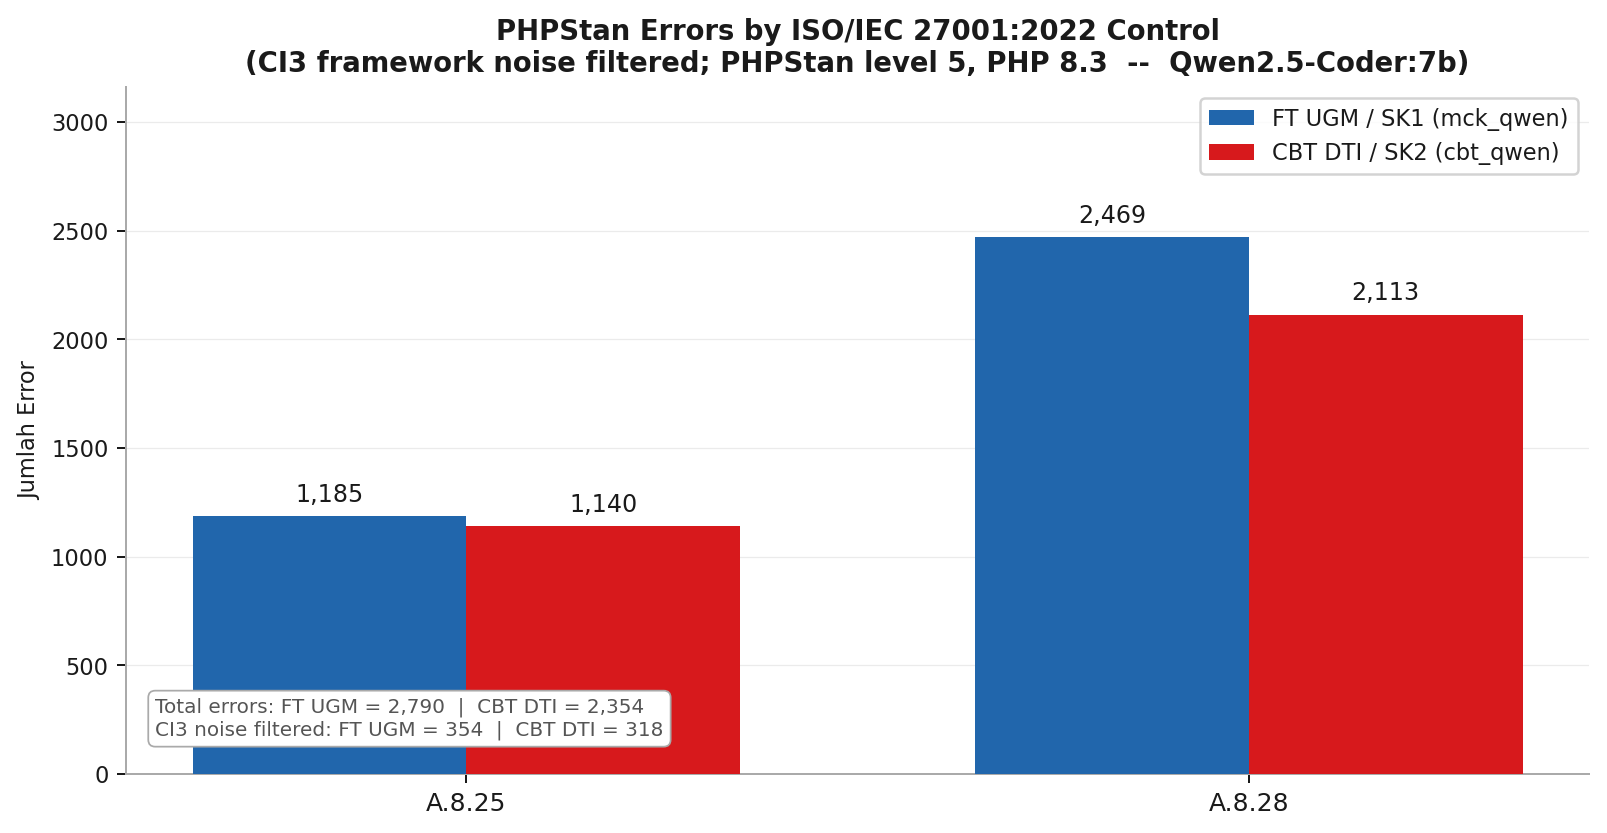
\includegraphics[width=0.9\textwidth]{contents/chapter-4/comparison/comparison_qwen_3_phpstan_iso.png}
    \caption{Comparison of PHPStan errors by ISO/IEC 27001:2022 control across both case studies}
    \label{fig:comparison-phpstan}
\end{figure}
\newpage
FT UGM produced 2,790 PHPStan errors while CBT DTI produced 2,354. Both were run on PHPStan level 5 targeting PHP 8.3, so the figures are directly comparable. The majority of errors in both datasets are false positives arising from PHPStan's limitations in tracing CodeIgniter 3.x's dynamic architecture, particularly magic properties and helper functions injected at runtime. Beyond those, a portion of the errors reflect genuine application code compatibility and quality issues, as discussed in the preceding sections.

The higher error count in FT UGM, despite its smaller dataset size (245 vs 326 files), is attributable to the use of more diverse third-party dependencies: PHPStan cannot resolve classes such as \texttt{PhpOffice\textbackslash PhpSpreadsheet} and \texttt{Dotenv\textbackslash Dotenv} because the dependencies are not fully installed in the analysis environment.

% ------------------------------------------------------------
\subsection{Summary Comparison and Composer Dependency Analysis}
% ------------------------------------------------------------

Table~\ref{tab:comparison-summary} summarizes all primary metrics from both case studies in a single view, including the FT UGM composer dependency status.

\begin{table}[h]
\caption{Summary comparison of pipeline metrics and composer dependency status across both case studies}
\vspace{0.5em}
\centering
\label{tab:comparison-summary}
\begin{tabularx}{\textwidth}{|>{\raggedright\arraybackslash}X|>{\centering\arraybackslash}p{3.6cm}|>{\centering\arraybackslash}p{3.6cm}|}
\hline
\textbf{Metric} & \textbf{FT UGM / CS1 (mck\_qwen)} & \textbf{CBT DTI / CS2 (cbt\_qwen)} \\
\hline \hline
PHP files analyzed & 245 & 326 \\
\hline
Semgrep findings (pre) & 11 & 11 \\
\hline
\hspace*{1em}-- SQL Injection & 1 & 1 (CI3 core) \\
\hline
\hspace*{1em}-- SSRF & 10 & 10 (CI3 core) \\
\hline
Semgrep delta (post--pre) & +0 (stable) & +0 (stable) \\
\hline
Rector converted & 239 (97.6\%) & 299 (91.7\%) \\
\hline
Rector skipped & 4 & 25 \\
\hline
Rector failed & 2 (Fiber bug) & 2 (Fiber bug) \\
\hline
PHPStan total errors & 2,790 & 2,354 \\
\hline
\hspace*{1em}CI3 noise filtered & 354 & 318 \\
\hline
AI recommendations & 11 (Qwen2.5-Coder:7b) & 11 (Qwen2.5-Coder:7b) \\
\hline
ISO overall status & NON-COMPLIANT & NON-COMPLIANT \\
\hline
Custom app code (Semgrep) & 0 findings & 0 findings \\
\hline
\end{tabularx}
\end{table}

\noindent PHPStan errors in both case studies are predominantly false positives from the CI3 framework (magic props, runtime constants). The Semgrep delta is 0 for both case studies because Rector neither introduces nor removes vulnerabilities. All detected Semgrep findings originate from \texttt{CI3 system/core/Output.php} and are not part of the custom application code.

Overall, both case studies exhibit a consistent pattern: the pipeline successfully executes all stages automatically, Rector's conversion produces syntactically valid code across both datasets, and the ISO/IEC 27001:2022 status for both is \texttt{NON\_COMPLIANT} driven by PHPStan errors. The primary differences lie in the Rector conversion rate (97.6\% vs 91.7\%), the number of PHPStan errors (2,790 vs 2,354), and the availability of composer dependency analysis: FT UGM has a \texttt{composer.json} file with five dependencies examined (three \texttt{SAFE}, two \texttt{MANUAL REVIEW}), while CBT DTI has no such file and the dependency analysis step is automatically skipped. In terms of execution duration, both case studies are comparable at approximately 3 to 4 minutes, because both use Qwen2.5-Coder 7b as the AI Engine with a single inference per finding; the multi-model comparison experiment (Conditions A through C) in the FT UGM case study is a separate evaluation procedure and is not included in the pipeline duration measurement.